%Copyright 2014 Jean-Philippe Eisenbarth
%This program is free software: you can 
%redistribute it and/or modify it under the terms of the GNU General Public 
%License as published by the Free Software Foundation, either version 3 of the 
%License, or (at your option) any later version.
%This program is distributed in the hope that it will be useful,but WITHOUT ANY 
%WARRANTY; without even the implied warranty of MERCHANTABILITY or FITNESS FOR A 
%PARTICULAR PURPOSE. See the GNU General Public License for more details.
%You should have received a copy of the GNU General Public License along with 
%this program.  If not, see <http://www.gnu.org/licenses/>.

%Based on the code of Yiannis Lazarides
%http://tex.stackexchange.com/questions/42602/software-requirements-specification-with-latex
%http://tex.stackexchange.com/users/963/yiannis-lazarides
%Also based on the template of Karl E. Wiegers
%http://www.se.rit.edu/~emad/teaching/slides/srs_template_sep14.pdf
%http://karlwiegers.com
\documentclass{scrreprt}
\usepackage{listings}
\usepackage{underscore}
\usepackage[bookmarks=true]{hyperref}
\usepackage[utf8]{inputenc}
\usepackage[english]{babel}
\usepackage{xcolor,colortbl}
\usepackage{makecell}
\usepackage{graphicx}
\hypersetup{
    bookmarks=false,    % show bookmarks bar?
    pdftitle={Software Requirement Specification},    % title
    pdfauthor={Jean-Philippe Eisenbarth},                     % author
    pdfsubject={TeX and LaTeX},                        % subject of the document
    pdfkeywords={TeX, LaTeX, graphics, images}, % list of keywords
    colorlinks=true,       % false: boxed links; true: colored links
    linkcolor=blue,       % color of internal links
    citecolor=black,       % color of links to bibliography
    filecolor=black,        % color of file links
    urlcolor=purple,        % color of external links
    linktoc=page            % only page is linked
}%
\newcolumntype{L}[1]{>{\raggedright\let\newline\\\arraybackslash\hspace{0pt}}m{#1}}
\newcolumntype{C}[1]{>{\centering\let\newline\\\arraybackslash\hspace{0pt}}m{#1}}
\newcolumntype{R}[1]{>{\raggedleft\let\newline\\\arraybackslash\hspace{0pt}}m{#1}}
\def\myversion{0.1 }
\definecolor{LightCyan}{rgb}{0.88,1,1}
\date{}
%\title
\usepackage{hyperref}
\begin{document}

\begin{flushright}
    \rule{16cm}{5pt}\vskip1cm
    \begin{bfseries}
        \Huge{SOFTWARE REQUIREMENTS\\ SPECIFICATION}\\
        \vspace{1.9cm}
        for\\
        \vspace{1.9cm}
        App FH++\\
        \vspace{1.9cm}
        \LARGE{Version \myversion}\\
        \vspace{1.9cm}
        Prepared by \\ {\small Mohamad Arastu, Raphael Arzberger, Martin Fuhrmann}
        \vspace{1.9cm} \\
        \today\\
    \end{bfseries}
\end{flushright}

\tableofcontents


\chapter*{Revision History}

\begin{center}
    \begin{tabular}{|c|c|c|c|}
        \hline
	    Date & Reason For Changes & Version\\
        \hline
	    14.09.2022 & project start & 0.1\\
        \hline
    \end{tabular}
\end{center}

\chapter{Introduction}

\section{Purpose}

The FH++ app, which is being developed as part of this software project, is intended to be a useful tool for students at the FH Campus Wien and is meant to be an addition to existing services like FH Portal and Moodle. \\ \\
The goal is to offer users of the app the opportunity to make their studies as efficient as possible.
By using the interfaces of the FH portal and those of the open data portal of the City of Vienna, which enables access to data from Wiener Linien,
the users should be empowered to plan their everyday studies in a time-optimizing manner.
The arrival at the FH can be planned by combining information from the individual timetable and current traffic data for public transport. \\
As an example, in case the metro U1 is used for getting to the FH, the app is intended to warn of a potentially later arrival time in the event of disruptions in the subway network.
For navigation within the FH building, the user should be able to use a navigation aid. \\
In addition, the app should also allow to read and send emails from the FH mail account.

\section{Organizational Embedding}
The project takes place as part of the ILV Software Engineering course. The students of the Vienna University of Applied Sciences should benefit from the application.

\chapter{Functional Requirements}

\section{Use Case Diagram}

\begin{figure} [h]
	\centering
	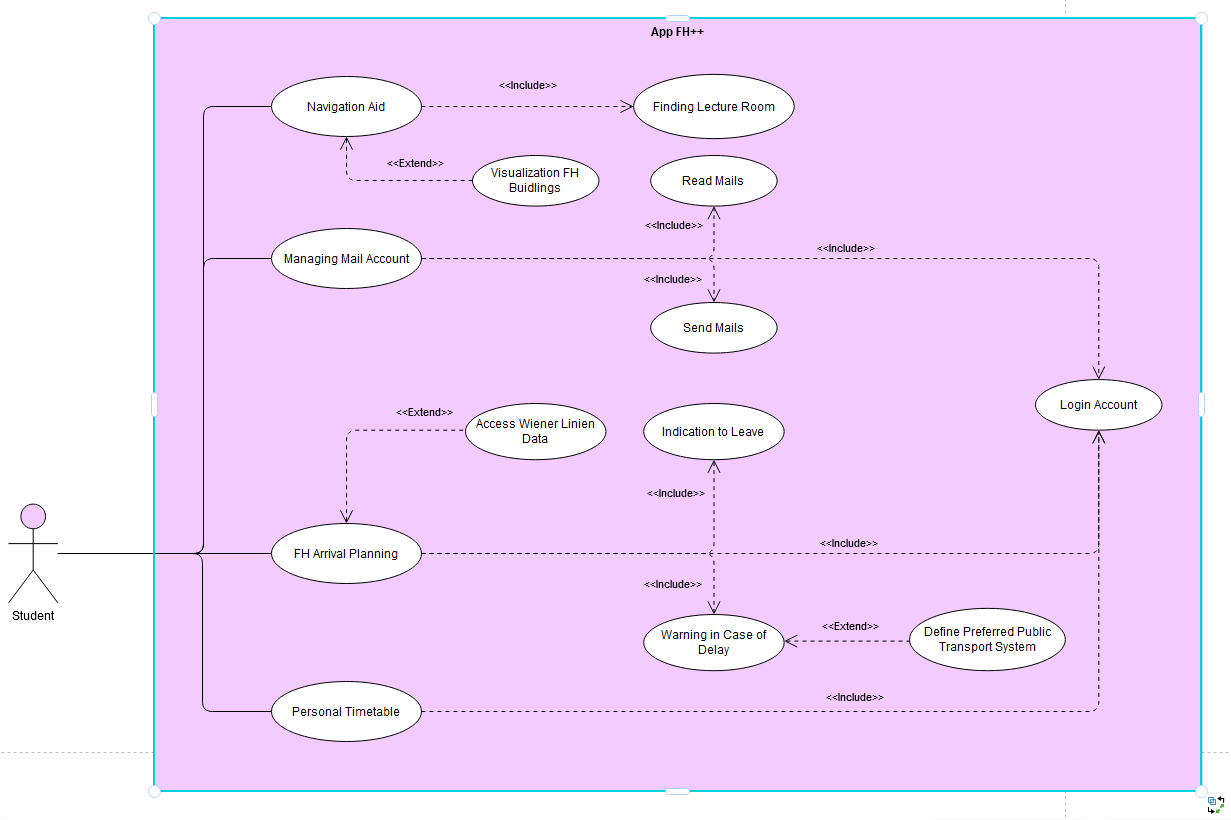
\includegraphics[width=1\linewidth]{pics/usecasediagram}
	\caption{Use Case Diagram}
	\label{fig:usecasediagram}
\end{figure}

\section{Use cases}
\begin{center}
\begin{tabular}{|L{2.1cm}|L{12cm}|l|}
	\hline
	\rowcolor{LightCyan}
	\rule[-1ex]{0pt}{2.5ex} Use Case & Navigation Aid / Room Search  \\
	\hline
	\rule[-1ex]{0pt}{2.5ex} Actors & {\small User} \\
	\hline
	\rule[-1ex]{0pt}{2.5ex} Description & {\small Specific facilities of the campus are visualized on a map.} \\
	\hline
	\rule[-1ex]{0pt}{2.5ex} Stimulus & \makecell[l]{{\small By clicking on the "show room" button } \\ {\small or by chosing the option "show room" option in the timetable feature.}} \\
	\hline
	\rule[-1ex]{0pt}{2.5ex} Response & \makecell[l]{{\small The desired room is highlighted in a visualization of buildings of the campus.}} \\
	\hline
	\rule[-1ex]{0pt}{2.5ex} Criteria & \makecell[l]{
		\textbf{MUST:} {\small Every room shall be depictable in a 3D map.} \\ {\small The user shall be able to rotate the virtualization of the buildings in all } \\ {\small axes and shall also be able to zoom in and out.} \\
		\textbf{SHOULD:} {\small The room search feature should interact with the timetable.} \\
		{\small If a lecture is visible in the timetable the app should provide the possibility } \\ {\small to show the lecture room in the virtualized campus map.} \\
		{\small lecture. In case of an online lecture a zoom link should be used instead } \\ {\small of the map.} \\
		\textbf{COULD:} {\small The navigation within the buildings could be implemented using } \\ {\small augmented reality.} \\
	}	\\
	\hline
	\rule[-1ex]{0pt}{2.5ex} Comments & {\small No login needed for this feature, except feature is opened up from within timetable. }  \\
	\hline
\end{tabular}
\begin{tabular}{|L{2.1cm}|L{12cm}|l|}
	\hline
	\rowcolor{LightCyan}
	\rule[-1ex]{0pt}{2.5ex} Use Case & FH Arrival Planning  \\
	\hline
	\rule[-1ex]{0pt}{2.5ex} Actors & {\small User } \\
	\hline
	\rule[-1ex]{0pt}{2.5ex} Description & {\small The user is informed when to leave in order to arrive at the FH in time.  } \\
	\hline
	\rule[-1ex]{0pt}{2.5ex} Stimulus & \makecell[l]{{\small Information from timetable, user settings, current location and } \\ {\small open data portal of the city of Vienna }} \\
	\hline
	\rule[-1ex]{0pt}{2.5ex} Response & \makecell[l]{{\small The user is informed by a notification alarm.}} \\
	\hline
	\rule[-1ex]{0pt}{2.5ex} Criteria & \makecell[l]{
		\textbf{MUST:} {\small Based on the stimulus mentioned above the user has to be } \\ {\small informed when to leave in order to arrive at the FH in time. By default } \\ {\small the fastest public transport system should be chosen. If desired by the } \\ {\small the user, a preferred public transport system can be configured.} \\
		\textbf{SHOULD:} {\small In case there are severe disruptions with the preferred public} \\ {\small transport system the app should inform the user and suggest alternative } \\ {\small routes.}} \\
	\hline
	\rule[-1ex]{0pt}{2.5ex} Comments & Login needed for this feature.  \\
	\hline
\end{tabular}
\begin{tabular}[h]{|L{2.1cm}|L{12cm}|l|}
	\hline
	\rowcolor{LightCyan}
	\rule[-1ex]{0pt}{2.5ex} Use Case & Managing Mail Account  \\
	\hline
	\rule[-1ex]{0pt}{2.5ex} Actors & {\small User } \\
	\hline
	\rule[-1ex]{0pt}{2.5ex} Description & {\small Read and write mails of the FH Campus Wien mail account. } \\
	\hline
	\rule[-1ex]{0pt}{2.5ex} Stimulus & \makecell[l]{{\small By clicking on the "email" button. }} \\
	\hline
	\rule[-1ex]{0pt}{2.5ex} Response & \makecell[l]{{\small The mail application should open up.}} \\
	\hline
	\rule[-1ex]{0pt}{2.5ex} Criteria & \makecell[l]{
		\textbf{MUST:} {\small The mail application shall be connected to the users' mail account.} \\ {\small The user shall be able to read and write mails.} \\
		\textbf{COULD:} {\small In case the user is running late there could be an option to allow } \\ {\small automatic notification of a predefined user group and or the lecturer about } \\ {\small the delay per mail.} \\
	}	\\
	\hline
	\rule[-1ex]{0pt}{2.5ex} Comments & Login needed for this feature.  \\
	\hline
\end{tabular}
\begin{tabular}{|L{2.1cm}|L{12cm}|l|}
	\hline
	\rowcolor{LightCyan}
	\rule[-1ex]{0pt}{2.5ex} Use Case & Timetable  \\
	\hline
	\rule[-1ex]{0pt}{2.5ex} Actors & {\small User } \\
	\hline
	\rule[-1ex]{0pt}{2.5ex} Description & {\small The user-specific timetable is displayed.  } \\
	\hline
	\rule[-1ex]{0pt}{2.5ex} Stimulus & \makecell[l]{{\small By clicking on the "timetable" button.}} \\ 
	\hline
	\rule[-1ex]{0pt}{2.5ex} Response & \makecell[l]{{\small The timetable is opened up.}} \\
	\hline
	\rule[-1ex]{0pt}{2.5ex} Criteria & \makecell[l]{
		\textbf{MUST:} {\small The user shall be able to view the timetable of the current semester. } \\ {\small The location of any lecture shall be shown on a map of the campus.} \\
		\textbf{SHOULD:} {\small The user should be able to see how long it takes to get from } \\ {\small current position to the lecture room. }} \\ 
	\hline
	\rule[-1ex]{0pt}{2.5ex} Comments & Login needed for this feature.  \\
	\hline
\end{tabular}
\end{center}

\chapter{Non-Functional Requirements}
\section{Requirements for data retention}
The application must comply with the DSGVO and Austrian laws and standards
correspond. An implementability of the corresponding guidelines of the DSGVO must be ensured, e.g. how long the data may be kept, whether the members
must take note of a privacy policy, that the data will not be passed on to third parties and that the data can be deleted upon request can be carried out.

\section{General description of the data}
The system must be expandable: new members and modules should be able to
be added, but also be able to be deleted. The names
of the modules and the names of the members should be changeable. Data must be
be checked for authenticity before they are added to the database.

\section{Performance requirement}
The data provided through the system must be refreshed immediately after a change happened: The user needs to be get the newest information within half a minute. Also refreshing the data on the app must not take longer than 10 seconds.

\section{Installation and Tutorial}
The application must be self-explanatory: The average user should be able to use the application with all its functions in a matter of 15 minutes. The context of the menu and the application as such, must be in a user-friendly, easy to understand way.

\section{Accessibility}
Accessible design must be integrated into the application: Text size, font, colours and menus must be tuned, as to enable as many people with accessibility difficulties as possible, to use the app in an efficient and easy way.

\section{Data security}
Login credentials and other sensitive information must be stored and transmitted only in a encrypted state. At no time in the system is any sensitive data allowed to be in cleartext. Modern up to date encryption must be used to ensure data safety.

\section{Multiple platforms}
The application must be available on all modern platforms to be useable by every student on every machine: to reach this goal the application must be compatible with the top ten modern browsers available at the moment.

\end{document}
